%%%%%%%%%%%%%%%%%%%%%%%%%%%%%%%%%%%%%%%%%%%%%%%%%%%%%%%%%%%%%%%%%%%%%%%%%%%%%%%%
%2345678901234567890123456789012345678901234567890123456789012345678901234567890
%        1         2         3         4         5         6         7         8

\documentclass[letterpaper, 12 pt, conference]{ieeeconf}  

% \IEEEoverridecommandlockouts
% This command is only needed if you want to use the \thanks command
\overrideIEEEmargins
% See the \addtolength command later in the file to balance the column lengths on the last page of the document



% The following packages can be found on http:\\www.ctan.org
\usepackage[final]{graphics} % for pdf, bitmapped graphics files
\usepackage{epsfig} % for postscript graphics files
\usepackage{mathptmx} % assumes new font selection scheme installed
\usepackage{times} % assumes new font selection scheme installed
\usepackage{amsmath} % assumes amsmath package installed
\usepackage{amssymb}  % assumes amsmath package installed
% \usepackage{caption}
% \usepackage{subcaption}

\title{\LARGE \bf
Interactive Robot Learning: Final Project Update 
}
\author{Pramodith B and Tanmay B}
\begin{document}
\maketitle
\thispagestyle{empty}
\pagestyle{empty}

%%%%%%%%%%%%%%%%%%%%%%%%%%%%%%%%%%%%%%%%%%%%%%%%%%%%%%%%%%%%%%%%%%%%%%%%%%%%%%%%
\begin{abstract}

Our project aims to teach an agent to stack blocks together in a simulated 2D world. We attempt to make the algorithm partially extensible to new goal configurations. This can be abstracted as teaching an agent how and where to move objects located in any environment. A physical robot that operates in the real world would need to have skills to move objects around it to complete complex tasks. We developed a Reinforcement Learning Algorithm which is independent of the starting locations of each block in the environment to teach the bot to stack blocks. We then make use of an Oracle and expert demonstrations to help the Reinforcement Learning Algorithm based on the hypothesis that the oracle and human demonstrations can help in correcting the agent and thereby improve its performance. 

\end{abstract}


%%%%%%%%%%%%%%%%%%%%%%%%%%%%%%%%%%%%%%%%%%%%%%%%%%%%%%%%%%%%%%%%%%%%%%%%%%%%%%%%
\section{INTRODUCTION}

The block world and block stacking tasks are classical AI problems. The general idea is that given a set of blocks in a real or simulated environment the agent needs to arrange blocks in a particular configuration. The problem can be abstracted to multiple levels. At a very high level of abstraction it can be deemed to be a planning problem that doesn’t require an environment of any sort. At a very low level it can be deemed to be a real world task in a continuous  state and action space with a physical robot trying to move the blocks to achieve the desired configuration.

Learning from human demonstrations and experts has become a very popular and effective technique in the world of robotics. Often the demonstrations narrow down the search space that the agent has to explore or provide it with good initialization parameters to start learning a task. Using experts to correct the actions of an agent also allows a sub optimal agent learn rapidly from it’s mistakes and perform much better at the task that it was built to perform.

We attempt to create an agent that can stack blocks in a 2D simulated world. We consider just 2 and 3 blocks in our environment and aim at building just one stack. We do not care about the location of the stack but just that the blocks are in the right order. We make use of Q-Learning to build a sub optimal agent. We developed  an analytical solution to the problem and treat it as an Oracle to help in correcting the sub-optimal agent. We also secured a few human demonstrations that correct the sub optimal agent when they think that it’s making a wrong move. We assess the performance of our agent and it’s improvement after using the oracle and human demonstrations.


\section{Related Works}

% \subsection{Selecting a Template (Heading 2)}

The block world environment and block stacking are classical AI problems. There have been plenty of approaches using planning, reinforcement learning with heavily hand crafted human rewards and more recently deep learning and deep reinforcement learning techniques to solve the problem.

Hohm, Egli et al \cite{hohm2007evolutionary} propose using evolutionary algorithms in order to stack blocks on a table to maximize the overhang. Overhang is the maximum distance between the table or surface that supports the block and the block that is the furthest away from the table along the horizontal axis.  Dzeroski, S., De Raedt et al\cite{dvzeroski2001relational} propose using reinforcement learning and inductive logic programming to generate plans to stack blocks.

More recently Deep Reinforcement learning techniques have come to the forefront in this domain of problems. The block stacking problem in a simulation world can be treated as a game where the agent is expected to learn a policy that can maximize the score it can achieve in the game.

Mnih, David et al's \cite{mnih2013playing} breakthrough paper propose a Deep Neural Net architecture that learns to play Atari games at a level comparable to humans. They call their model the Deep Q Network since the Neural Net Approximates the Q function that they intend to learn. They make use of the learnt Q function to pick an action to perform at every state of the game thereby obtaining the policy. The same authors proposed a technique called experience replay to come up with a training strategy that doesn't break the IID assumption that’s often made while applying Machine Learning Algorithms. Games almost always have a sequence and training a DQN on sequences of consecutive frames would violate the IID principle and lead to ineffective learning. 

Li et al \cite{DBLP:journals/corr/abs-1711-00267} proposed a method to use a Deep Q Network with a changing goal for every instance of a 2D block stacking game. They propose making the goal a part of the state that is fed as input to the Deep Q Network. However all the Deep Q Learning algorithms require very large amounts of data to be trained successfully. Hester, Vecerick et al.\cite{hester2017deep} propose a new loss function that takes into consideration what the  demonstrator has done at a particular state. This allows the Deep Q Network to learn effectively from human demonstrators while requiring less data.

Abeel et al\cite{duan2017one} successfully taught a robot arm in simulation and in a real world environment to create multiple stacks of blocks given a goal configuration, that specified the number of stacks and the blocks that form each stack based on human demonstrations. They propose a new Deep Learning Network that makes use of a 2-stage-attention network to learn to focus on important time frames of demonstrations and on the important blocks. This approach allows them to perform One Shot Imitation Learning since a trained model can successfully reach a new goal configuration given just one demonstration but with a different starting state.


\section{Methodology}

In this section, we elaborate our attempted approaches and report why they succeeded or failed. Our goals for the project gradually changed as we learnt of various limitations and encountered problems that were too difficult to solve in the given time frame.

Initially, we wanted to follow the approach of "One Shot Imitation Learning" by Abeel et al\cite{duan2017one}. We experimented with OpenAI’s Gym\cite{openaigym} environment which simulated a robotic arm controlling a 3D block world environment. However, we were ineffective in using the environment to actively obtain demonstrations from a user using a keyboard or controller since the physics engine (Mujoco\cite{mujoco}) was listening to all events and provided no method to augment it.

Following which, we moved onto creating our own 3D environment using two javascript libraries called Three.js \cite{threejs}(3D world) and Cannon.js\cite{cannonjs} (Physics engine). Here we faced difficulties with the physics and the mapping of the 2D input(screen) to the 3D world. This made it difficult to provide successful demonstrations. We also realized that the architecture required by Abeel et al\cite{duan2017one} required hundreds of thousands of examples to be trained successfully.

\begin{figure}
\subfloat{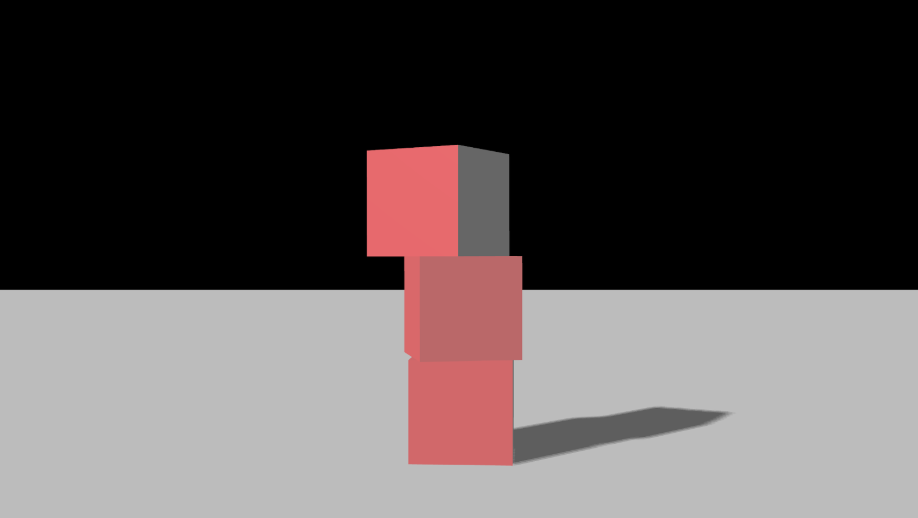
\includegraphics[width = 1.5in]{3d-blocks.png}}
\subfloat{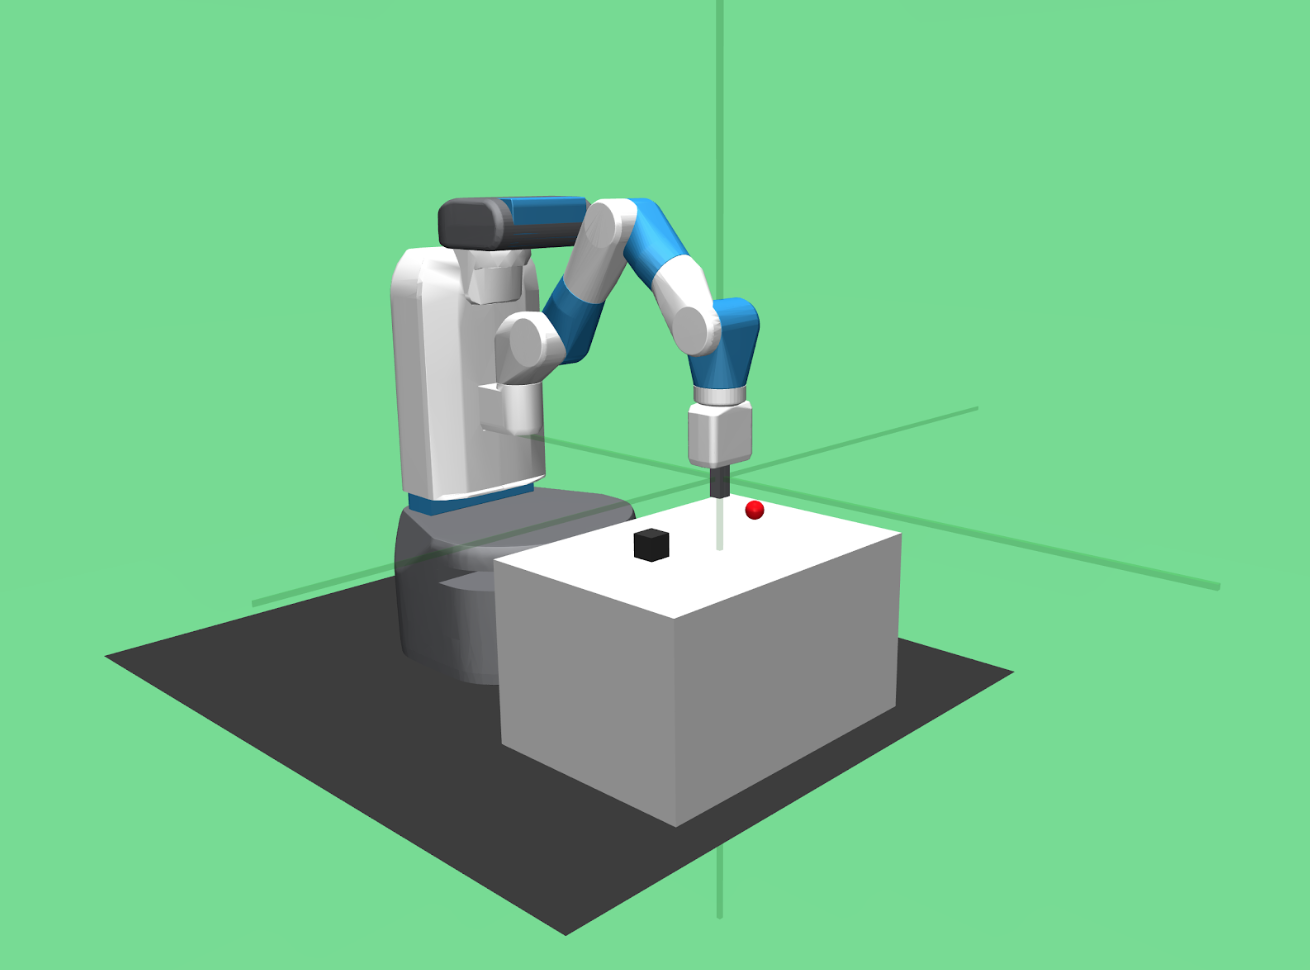
\includegraphics[width = 1.5in]{openai.png}}
\caption{left: 3d Block world; right: OpenAI Gym's robotic arm}
\label{preenvs}
\end{figure}

As a result we decided to simplify our problem further by moving to a 2D environment and treat the block stacking problem as a simple Atari game and make use of Deep Q networks to obtain a policy.

\subsection{2D Environment} We developed a 2D simulation environment using PyGame\cite{pygame}. The 2D environment has no physics involved and can be thought of as a table with blocks when viewed from the top. 
Allowing the blocks to be placed on every pixel coordinate caused an explosion of state space. We hence limit our actions to take large steps that are equal to the size of the block length
The environment is divided into grids of a step size equal to the size of the block. The entire environment is a 7 $\times$ 7 grid. Each block in the environment is associated with a unique color. The action space is 

\begin{itemize}
    \item Move Up
    \item Move Down
    \item Move Left
    \item Move Right
    \item Pick (Block Id)
    \item Drop
\end{itemize}
The goal configuration is depicted as a small 70 * 70 image at the top right corner of the game screen.
This results in a state space of $$ ^{7 \times 7}C_{\text{Block Count}} \times |A| = 3,31,632 $$ for 3 blocks.

\begin{figure}[thpb]
  \centering
  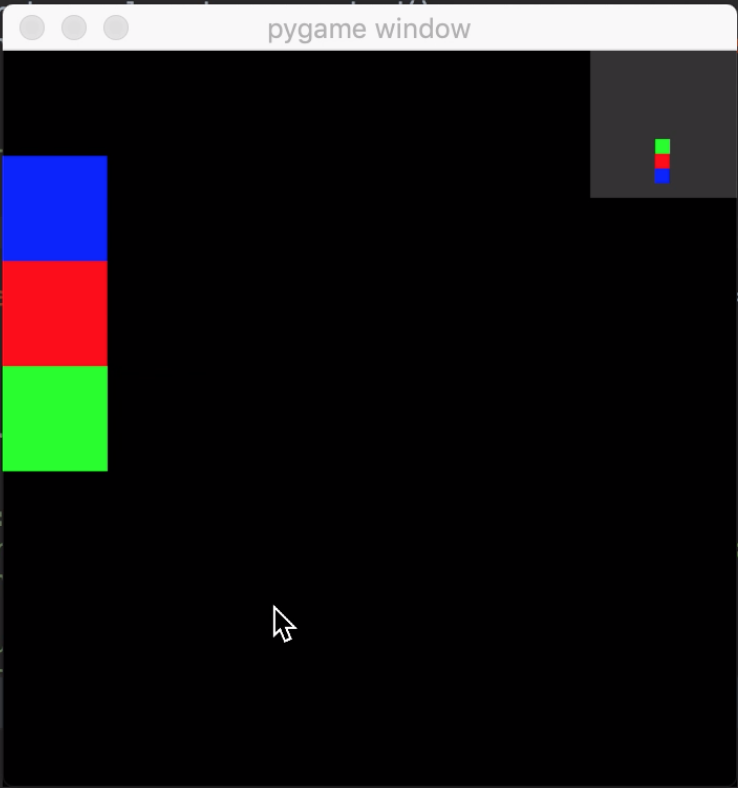
\includegraphics[scale=0.5]{blockworld.png}
  \caption{2d Block World Demonstration Environment}
  \label{figurelabel}
\end{figure}

\subsection{Preliminaries}
\subsubsection{Markov Decision Processes }
A Discrete Markov Decision Process is a 5-tuple $(S, A, P_a, R_a, \gamma)$, where
\begin{itemize}
    \item $S$ is a finite set of states
    \item $A$ is a finite set of actions (alternatively, $A_{s}$ is the finite set of actions available from state $s$)
    \item $P_{a}(s,s')=\Pr(s_{t+1}=s'\mid s_{t}=s,a_{t}=a)$ is the probability that action $a$ in state $s$ at time $t$ will lead to state $s'$ at time $t+1$
    \item $R_{a}(s,s')$ is the immediate reward (or expected immediate reward) received after transitioning from state $s$ to state $s'$, due to action $a$
    \item$\gamma$ is the discount factor
\end{itemize}

\subsubsection{Q-Learning} 
The  Q function defines the expected reward for every state, action pair. At test time, the argmax of the q values at a state determines the action that the agent should take to maximize the reward(or minimize the cost)
Before learning begins, $ Q$ is initialized to a possibly arbitrary fixed value (chosen by the programmer). Then, at each time $ t$ the agent selects an action $a_{t}$, observes a reward $r_{t}$, enters a new state $ s_{t+1} $ (that may depend on both the previous state $s_{t}$  and the selected action), and $Q$ is updated. The core of the algorithm is a simple value iteration update, using the weighted average of the old value and the new information:
\begin{align}
    Q(s_, a_t) &\leftarrow (1-\alpha)Q(s_t, a_t) \nonumber\\ 
              &+ \alpha (r_t + \gamma (max_a Q[s_{t+1}, a])) 
\end{align}

where $r_{t}$ is the reward received when moving from the state $ s_{t}$ to the state $s_{t+1}$, and $ \alpha $  is the learning rate ( $0<\alpha \leq 1$
The discount factor determines the importance of future rewards. With a lower discount factor, the agent focuses more on short term reward over long term rewards. 

The learning rate determines the importance of newly obtained information. A higher value of $\alpha$ forces the agent to learn more from the newly visited states over the existing q values

We also use an epsilon greedy approach while choosing actions at training time. $\epsilon \in [0, 1]$ determines the probability that the action taken is chosen from the best available q values in the current state over a randomly chosen action. With a lower value of $\epsilon$, the agent chooses more random actions than optimal actions suggested by the q table. This is useful so that the agent explores more states and learns to generalize better. 

\subsection{Deep Q Learning}
Deep Q learning attempts to use Deep Neural Networks to approximate the desired Q function. The networks input is a series of images from the game. The entire image is treated as the state. Each image should be associated with a reward value the reward can be explicitly fed in or can be implicitly present in the image, as the score that is displayed on the game screen. The network outputs a score for each possible action and this maps to the Q table values for each action in the current state.

$$    \nabla_{\theta_{i}} L_i (\theta_{i}) = \mathbb{E}_{s,a\sim\rho(\cdot), s'\sim\epsilon} [( r + \gamma \max_{a'}Q(s', a'; \theta_{i-1} ) $$
$$ - Q(s, a; \theta_i)) )  \nabla_{\theta_{i}} Q(s, a; \theta_i) ]
$$

\subsubsection{Dataset and Preprocessing}
We procured the dataset using the following 2 methods:
\begin{itemize}
    \item Allowing the DQN to play the game and generate the action to make at the current state and then learn based on the reward it obtains after every action.
    \item We recorded a series of demonstrations for different goal configurations and passed the saved frames and the associated action and reward at that state to the DQN.
\end{itemize}

The entire image is scaled down to a 100 $\times$ 100 image before it is passed to the DQN. Unlike traditional approaches where the RGB images are converted to a grayscale image we maintain the three channels to ensure that color information is retained. In order to let the DQN observe which block to pick we also change the color of the picked block to white and set it back to its original color when it is dropped.

\subsubsection{Reward Function}

We experimented with two sets of rewards:
\begin{itemize}
    \item A sparse reward where a reward of +10 was given for reaching the goal configuration.
    \item A dense reward where a reward of (Current Distance between blocks/Maximum possible euclidean distance between blocks) for every state and a reward of +10 for reaching the goal configuration. We used Manhattan distance as the distance metric.
\end{itemize}

\subsubsection{Experience Replay}
Experience replay was suggested by Mnih, David et al\cite{mnih2013playing} as a technique to avoid violating the IID assumption when training a Deep Q Network. Instead of training the network on a sequence of frames, we store the last n states that the agent has experienced in a buffer and then randomly choose k states from the buffer and their corresponding rewards, actions and next states to perform a gradient update.

We built a Deep Q Network with the following architecture:
\begin{itemize}
    \item 2D Convolution Layer with 16 filters of size 8x8 and stride of 4
    \item 2D Convolution Layer with 32 filters of size 4x4 and stride of 2
    \item Two linear layers
\end{itemize}

Apart from the last linear layer each layer was succeeded by a ReLU activation function. Each convolutional layer is succeeded by a Batch Normalization Layer. We use a relatively large filter and stride length since the environment is sparse in terms of the amount of information each image can have, since a large part of the image is empty. 
We also make use of two networks called the target network and policy network. The target network is used to predict the Value of the next state V(s-next)  whereas the Policy network predicts the Q values of the current state Q(s-current,a) for all actions. After every iteration of the policy networks parameters gradients are updated whereas the target networks gradients are updated periodically to the policy networks parameters after every n epochs. We chose n to be 3 and 5 in our experiments. 

Having two networks and training them in such a manner stabilizes training and is supposed to make training faster since the target values that the policy network is  chasing aren't getting updated along with the policy network.

\subsubsection{Training}

We used a batch size of 64 and a buffer size of 1000. We experimented with MSELoss and Huber Loss and used the RMSprop optimizer with a learning rate of 1e-4. We also experimented with gradient clipping and learning rate delay.
For training we used a 2 tiered approach where we would
Train the network on the demonstrations
We  train this network further by letting it play the game and learn.
While training the network on demonstrations we added an extra loss term as suggested by Hester, Vecerick et al\cite{hester2017deep}.
The extra loss term was:
$$ J_E(Q) = \max_{a \in A} [Q(s, a) + l(a_E, a)] - Q[s, a_E] $$

Here a is the set of all actions chosen by the network and $a_e$ is the action taken by the expert demonstrator. S is the state and $l(a_e,a)$ is some arbitrarily chosen small constant value like 1 or 0.5 when $a_e$ and a are different and 0 when both are the same. The idea is to maximize the margin between the action taken by the expert and any other action chosen by the network.

We trained the network with different sets of hyper parameters for periods spanning 2-8 hours.
\subsubsection{Results}

The network didn't seem to learn anything apart from picking a block, after picking the block it seemed to take random actions. It was hard to debug and analyze since the loss values was stable, constant and small despite trying out different learning rates.


\section{Approach 2: Q-Learning}
We decided to move onto a normal Reinforcement Learning algorithm. We decided to use Q-Learning since we wanted to find how good each action was for a given state. We changed our state representation gradually as we observed different problems with our initial state representation.

\subsubsection{State representation 1}

We started with a vanilla state representation of the defined problem. Our state space contained the location of each block and another field denoting the index of the selected block. 
i.e. for a system with 3 blocks and the state is ($(x_1, y_1), (x_2, y_2), (x_3, y_3),$ selectedIndex) 

We realized that this state representation wouldn't work for changing goal locations and configurations. Since different goal configurations at different locations will have different policies we can't have a single policy that adapts well to all cases with the state representation mentioned above. 

We wanted to avoid training our agent on every possible goal location and configuration. It’s worthy to note that our goal is to reach a particular goal configuration. i.e.(Green , Blue, Red) where Green is on the bottom and the Red Block is on top but we do not enforce a location for the stack on the screen. 

To remove the dependency on goal location, and to accommodate different goals we defined our state space as:

(Total Pairwise Distance between blocks, Direction, Selected Block, Goal config)

Using such a representation lets the agent learn that it needs to reduce the distance between blocks. Direction represents the direction of the closest block to the picked block. It’s a simple tuple indicating whether the closest block is Up/Down and Left/Right relative to it. Goal config represents the goal configuration we want the agent to reproduce. Since the agent needs to just learn to reduce the distance between blocks the agent no longer depends on the location of the goal.

While this representation reduced the effective search space we still had to train the model on every possible goal configuration. To avoid this we came up with another state representation that makes the algorithm partially extensible to new unseen goal configurations.

(Distance to Target Block, Total pairwise distance between blocks, Direction of target block, Picked block index, (Source , Target)).

\subsubsection{Distance to chased block} In our scheme we reduced the entire problem to pairs of blocks chasing each other. So assuming the goal configuration is (0,1) it means that 0 is chasing the bottom of 1 and 1 is chasing the top of 0. If the goal configuration is (0,1,2) 0 will chase 1, 1 will chase 2 and 2 will chase the top of 1.
The first entry in the state is the distance between the picked block and the block that its supposed to chase.

\subsubsection{Total Pairwise distance} If the goal was 0,1,2 this would be the sum of the distances from 0 to 1 and from 1 to 2. Note that the distance from 0 to 2 is not involved since it’s redundant.

\subsubsection{Direction of chased block} Assuming that 1 is the picked block and 2 is the block that it is chasing it is the direction of 2 relative to 1. It’s a three-tuple where the first two tuples indicate Up/Down and Left/Right and the third entry indicates whether the cell below 2 is blocked off (i.e. occupied by another block) or not. 

\subsubsection{Source,Target} Source is the block that is chasing and target is the block that is being chased.
This representation is partially extensible to new goals since if the agent was trained on the goal configurations [0,2,1],[1,0,2] the agent should ideally be able to reach the goal [2,1,0] since it has been trained to let 2 chase 1 and 1 chase 0.

\subsubsection{Reward Function} After tuning the rewards to get good performance our reward structure was as follows:

\begin{itemize}
    \item A reward after every action.
    \begin{itemize}
        \item 1 if the distance between the target block and the picked block is chasing has reduced
        \item -5 if the distance between the target block and the picked block is chasing has increased
        \item 0 if no change in the distance
    \end{itemize}
    \item A reward of +5 for every pair of blocks that are adjacent to each other
     \item A reward of -0.1 for dropping a block if the distance between the block it’s chasing is greater than 5000
    \item A reward of -0.1 if the agent just picks and drops blocks
    \item A reward of 50 for every matching pair of block according to goal configuration
i.e. if the goal configuration is [1, 0, 2] and 0 is above 1 the agent receives a reward of 50. It receives an additional reward of 50  totalling to 100 if 2 is on top of 0
\end{itemize}

\section{Oracle}
The Oracle is built as an analytical solution to solve the 2D block world problem. We intended to use the Oracle to analyse the improvement of the RL Algorithm in terms of the number of steps that it takes to reach the goal. Apart from a few cases the oracle provides a path to reach the goal in the optimal number of steps.

The oracle takes as input an initial state and a goal configuration. On initialization, it finds the most optimal goal location based on its inputs. On every invocation of the \textit{get next action} for a state and a block, the Oracle returns an action for the specified block.  

\subsection{Goal Location}
To compute the optimal goal configuration, we find the grid location closest to the centroid of all the blocks. This can be used as the goal location of the central block when the number of blocks is odd. With a slight modification, this works for even number of blocks also. The remaining blocks are now assigned a goal position based on their relative location with the centroid.

\subsection{Algorithm}
For every block, given the goal location, the algorithm provides the action to reduce the distance to the goal, i.e. if the goal is to the left of the block, the algorithm returns a Action.LEFT and so on. If a block cannot get to the goal state, but is blocking other blocks, it is moved to a position that does not block other blocks. If there is no feasible action for a block we choose the DROP action, so that the other blocks blocking the given block move away and allow for this block to be moved in a subsequent iteration. 
In essence, we pick an action to move towards the goal, if that is not possible, we pick an action that will unblock others to move towards their goal location. 

\section{Experiments}

We limited our experiments to just  a single stack of 2 and 3 blocks. The blocks can start off at any position within the 7 x 7 grid. We trained the Q- Learning algorithm with an $\alpha$ of 1, a $\gamma$ of 0.1 and a $\epsilon$ value of 0.1. 
At test time, we use the trained Q-table to return the action to take with a probability of 0.9 and we pick an action at random with a probability of 0.1. We observed that the agent tends to oscillate between states such as choosing to always pick and drop the same block. Adding this randomness helped us escape these oscillating states. We believe that these oscillations are because the agent hasn't been trained long enough or our reward structure wasn't definitive enough for the agent.


\subsection{2-Block world}
On running the agent taking random actions for 100 games, the agent failed 4 times (horizon length = 1000) with an average of 263.55 actions to reach the goal state.

Training the agent with a pure RL algorithm, the agent took 75.25 steps for a $\nu$ of $\nu = 0.01$ and 77.92 steps for $\nu = 0.05$


\subsection{3-Block world}

We conducted experiments to analyze the effect of number of training games on the performance of the agent. We use the number of failures and number of steps to reach the goal as a measure of the performance.


\begin{figure}
\subfloat{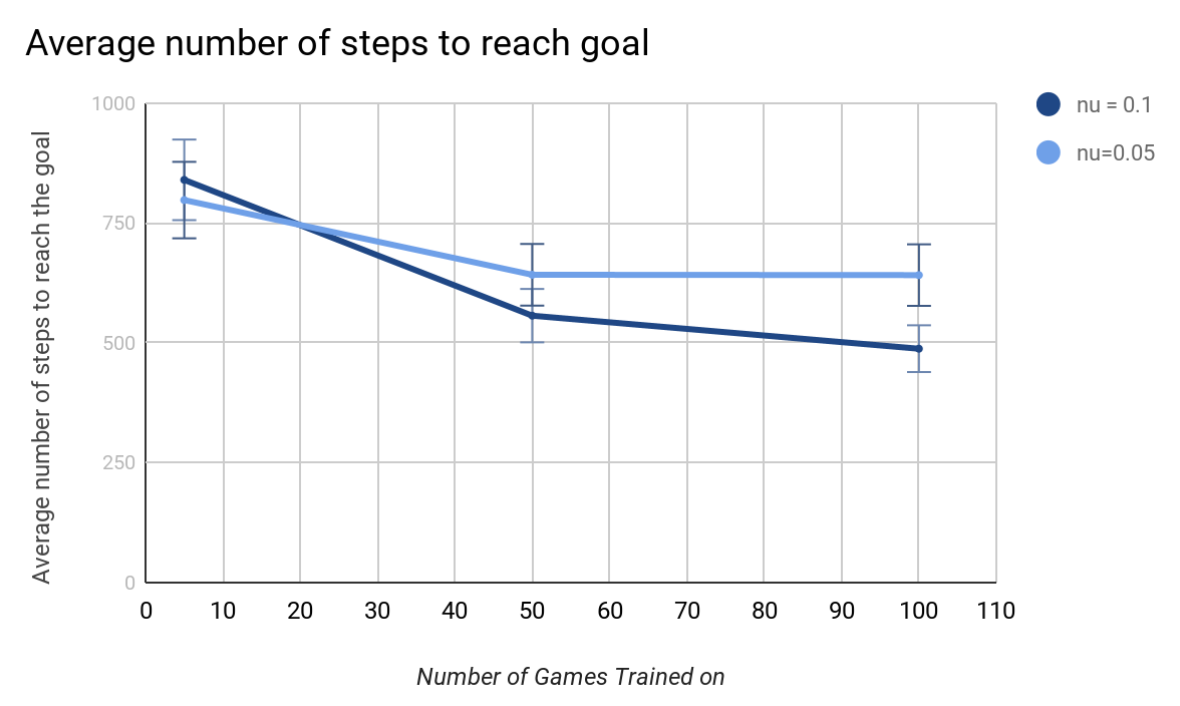
\includegraphics[width = 3in]{3b-avg-steps.png}}
\subfloat{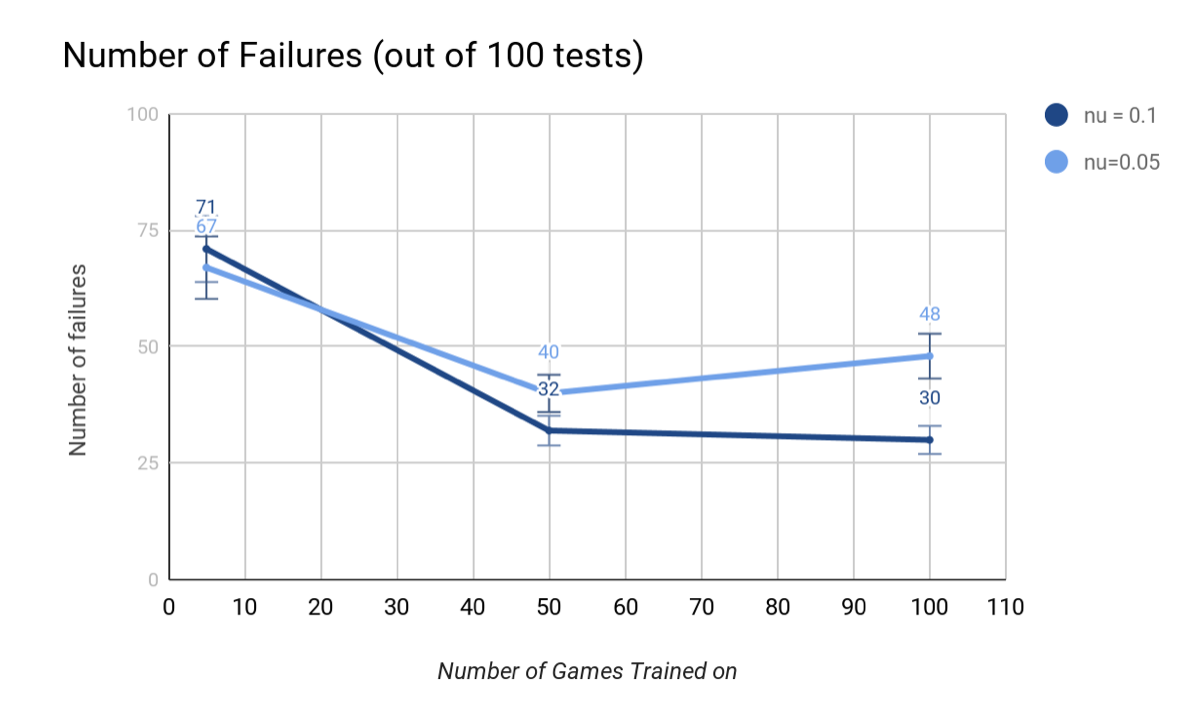
\includegraphics[width = 3in]{3b-avg-num-fail.png}}
\caption{Performance of 3 Block world} 
\label{perf}
\end{figure}


\subsubsection{Extensibility}

We conducted an experiment to check if the algorithm does partially extend to new goals that it hasn’t seen during train time. We trained the agent on the goals [[0,1,2],[1,0,2],[2,0,1],[0,2,1]]
And during test time we tested the agent on the goals [[2,1,0],[1,2,0]]. The agent failed to reach the goal 70 times out of 100 tries and took an average of 847.7 steps to reach the goal.
We then tested a completely random algorithm to reach the aforementioned 2 goal states we observed that the random algorithm achieved the goal just 3 times ie it failed 97 times out of 1000 and the average number of steps to success was 984.4. 

To test the statistical significance of this observation we used the Kolmogorov-Smirnov test since it’s a non parametric test that indicates whether the data points from 2 different samples are from the same distribution or not, it makes no assumptions about the distribution of the data like t-test and z-tests do. Our data didn't appear to be Gaussian either. The test indicated that the significance was 0.0993. So we could reject the null hypothesis that the differences in the means of the  convergence rates don’t come from the same distribution with a confidence of 90\%. 

From here on we will use the Wilcoxon test to assess whether the samples are from the same distribution or not. Wilcoxon is also non parametric and is said to be a better metric than Kolmogrov-Smirnov since it does not deviate more at the center as Kolmogrov does.It also does not assume that the underlying distribution is continuous.

\subsubsection{Oracle}

On noticing that our agent oscillated between states we believed that using the oracle to guide the agent during training whenever it oscillates between states and also randomly choosing to query the oracle would improve the agents performance. Table 1 shows the results observed, for oscillations we checked if the same pairs of actions occurred 3 times in a row and then queried the oracle. It indicates that we  can be confident that using the oracle when the agent is oscillating and also querying it with a probability of 0.1 helps the agent reach the goal quicker and also ensures fewer failures as compared to without using it.

\begin{table} [ht!]
    \caption{Oracle assistance performance}
    \begin{center}
        \begin{tabular}{|p{1.8cm}|p{1cm}|p{2cm}|p{2cm}|} 
            \hline
            Experiment Type & Number of failures out of 500 & Average number of steps to reach goal & Wilcoxon pvalue against baseline \\
            \hline
            Baseline & 186 & 578.626 & NA \\
            \hline
            Query the oracle during oscillation & 157 & 554.322 & 0.3395\\
            \hline
            Query during oscillation + 0.1 prob of choosing action decided by oracle & 125 &  518.668 &  0.016 \\
             \hline
        \end{tabular}
    \end{center}
\end{table}

\subsection{Trained Agent vs Demonstrators}
\subsubsection{Experimental Design}
We next decided to make use of demonstrations from humans to correct the agents behaviors. During test time we would often observe that the agent tended to get stuck in states or would oscillate between states we hypothesized that using demonstrators that could correct the agent when they believed that the agent was doing something wrong would help in improving the agents performance.

As part of our experimental design, we decided to provide the demonstrators with a trained RL agent. The demonstrator could stop the agent at any given time and choose an action that they think that the agent should do. The agent’s Q-table is updated during the demonstrations. Each demonstrator was asked to give 10 demonstrations in total. However, we restricted the total goal configurations that the user demonstrates on to just 4 out of the possible 6, since we wanted to see how well the agent can generalize

Table II indicates that after demonstrations the agent's corresponding to each demonstrator improved in terms of the number of times the agent succeeded in reaching the goal and also attained the goal faster than the baseline. However it appears like only the results of the first 2 demonstrators are statistically significant.

\begin{table}[ht!]
    \caption{All goals}
    \begin{center}
        \begin{tabular}{|p{2cm}|p{1cm}|p{2cm}|p{2cm}|} 
            \hline
             & Failures out of 500 & Average number of steps to reach goal & Wilcoxon Signed Rank Test \\ \hline
            Baseline & 160 & 534.35 & NA \\  \hline
            Demonstrator 1 & 101 & 415.14 & 1.16e-05  \\  \hline
            Demonstrator 2 & 107 & 419.212 & 3.23e-06 \\  \hline
            Demonstrator 3 & 113 & 453.83 & 0.0013 \\ \hline
        \end{tabular}
    \end{center}
\end{table}

Our next couple of experiments were aimed at finding how well the agent performed on the goals that the demonstrators hadn't corrected it on. Both the tables are inconclusive some show very little improvement while others show deprecation, but the statistical tests seem to indicate that all the improvements aren't significant enough to draw a positive conclusion. This result is a bit surprising.
\begin{table}[ht!]
    \caption{Unseen fixed goal [0,2,1]}
    \begin{center}
        \begin{tabular}{|p{2cm}|p{1cm}|p{2cm}|p{2cm}|} 
            \hline
             & Failures out of 500 & Average number of steps to reach goal & Wilcoxon pvalue against baseline \\ \hline
            Baseline & 96 & 398 & NA \\  \hline
            Demonstrator 1 & 124 & 454.574 & 0.022(Reject) \\  \hline
            Demonstrator 2 & 102 & 405.414 & 0.976 \\  \hline
            Demonstrator 3 & 82 & 387.644 & 0.957 \\ \hline
        \end{tabular}
    \end{center}
\end{table}
\begin{table}[ht!]
    \caption{Unseen fixed goal [2,0,1] during demonstrations}
    \begin{center}
        \begin{tabular}{|p{2cm}|p{1cm}|p{2cm}|p{2cm}|} 
            \hline
             & Failures out of 500 & Average number of steps to reach goal & Wilcoxon pvalue against baseline \\ \hline
            Baseline &  148 & 498.28 & NA  \\ \hline
            Demonstrator 1 & 143 & 510.418 & 0.811  (cannot reject h0) \\  \hline
            Demonstrator 2 & 152 & 520.962 & 0.449  (cannot reject h0)\\  \hline
            Demonstrator 3 & 122 & 457.596 & 0.123 (cannot reject h0) \\ \hline
        \end{tabular}
    \end{center}
\end{table}

\section{Conclusion}
When we started off the project we aimed at implementing an agent that could perform one shot imitation learning in a 3D environment. However after assessing the difficulty and obstacles of implementing such an agent we built an agent that can create stacks of size 2 and 3 blocks in a 2D environment. We initially tried to implement a Deep Q Network, but it failed to produce any sort of promising results. We finally settled on using Q learning to teach the agent. Our experiments show that the agent is partially extensible to unseen goals and corrective human demonstrations can help in teaching the agent and improve its performance both in terms of number of times the agent succeeds in building a stack corresponding to the right configuration and in terms of the number of steps the agent takes to reach the goal.

% \begin{itemize}

% \item Use either SI (MKS) or CGS as primary units. (SI units are encouraged.) English units may be used as secondary units (in parentheses). An exception would be the use of English units as identifiers in trade, such as Ò3.5-inch disk driveÓ.
% \item Avoid combining SI and CGS units, such as current in amperes and magnetic field in oersteds. This often leads to confusion because equations do not balance dimensionally. If you must use mixed units, clearly state the units for each quantity that you use in an equation.
% \item Do not mix complete spellings and abbreviations of units: ÒWb/m2Ó or Òwebers per square meterÓ, not Òwebers/m2Ó.  Spell out units when they appear in text: Ò. . . a few henriesÓ, not Ò. . . a few HÓ.
% \item Use a zero before decimal points: Ò0.25Ó, not Ò.25Ó. Use Òcm3Ó, not ÒccÓ. (bullet list)

% \end{itemize}


% \subsection{Equations}

% The equations are an exception to the prescribed specifications of this template. You will need to determine whether or not your equation should be typed using either the Times New Roman or the Symbol font (please no other font). To create multileveled equations, it may be necessary to treat the equation as a graphic and insert it into the text after your paper is styled. Number equations consecutively. Equation numbers, within parentheses, are to position flush right, as in (1), using a right tab stop. To make your equations more compact, you may use the solidus ( / ), the exp function, or appropriate exponents. Italicize Roman symbols for quantities and variables, but not Greek symbols. Use a long dash rather than a hyphen for a minus sign. Punctuate equations with commas or periods when they are part of a sentence, as in

% $$
% \alpha + \beta = \chi \eqno{(1)}
% $$

% Note that the equation is centered using a center tab stop. Be sure that the symbols in your equation have been defined before or immediately following the equation. Use Ò(1)Ó, not ÒEq. (1)Ó or Òequation (1)Ó, except at the beginning of a sentence: ÒEquation (1) is . . .Ó

% \subsection{Some Common Mistakes}
% \begin{itemize}

% \item The word ÒdataÓ is plural, not singular.
% \item The subscript for the permeability of vacuum ?0, and other common scientific constants, is zero with subscript formatting, not a lowercase letter ÒoÓ.
% \item In American English, commas, semi-/colons, periods, question and exclamation marks are located within quotation marks only when a complete thought or name is cited, such as a title or full quotation. When quotation marks are used, instead of a bold or italic typeface, to highlight a word or phrase, punctuation should appear outside of the quotation marks. A parenthetical phrase or statement at the end of a sentence is punctuated outside of the closing parenthesis (like this). (A parenthetical sentence is punctuated within the parentheses.)
% \item A graph within a graph is an ÒinsetÓ, not an ÒinsertÓ. The word alternatively is preferred to the word ÒalternatelyÓ (unless you really mean something that alternates).
% \item Do not use the word ÒessentiallyÓ to mean ÒapproximatelyÓ or ÒeffectivelyÓ.
% \item In your paper title, if the words Òthat usesÓ can accurately replace the word ÒusingÓ, capitalize the ÒuÓ; if not, keep using lower-cased.
% \item Be aware of the different meanings of the homophones ÒaffectÓ and ÒeffectÓ, ÒcomplementÓ and ÒcomplimentÓ, ÒdiscreetÓ and ÒdiscreteÓ, ÒprincipalÓ and ÒprincipleÓ.
% \item Do not confuse ÒimplyÓ and ÒinferÓ.
% \item The prefix ÒnonÓ is not a word; it should be joined to the word it modifies, usually without a hyphen.
% \item There is no period after the ÒetÓ in the Latin abbreviation Òet al.Ó.
% \item The abbreviation Òi.e.Ó means Òthat isÓ, and the abbreviation Òe.g.Ó means Òfor exampleÓ.

% \end{itemize}

% \section{USING THE TEMPLATE}

% Use this sample document as your LaTeX source file to create your document. Save this file as {\bf root.tex}. You have to make sure to use the cls file that came with this distribution. If you use a different style file, you cannot expect to get required margins. Note also that when you are creating your out PDF file, the source file is only part of the equation. {\it Your \TeX\ $\rightarrow$ PDF filter determines the output file size. Even if you make all the specifications to output a letter file in the source - if you filter is set to produce A4, you will only get A4 output. }

% It is impossible to account for all possible situation, one would encounter using \TeX. If you are using multiple \TeX\ files you must make sure that the ``MAIN`` source file is called root.tex - this is particularly important if your conference is using PaperPlaza's built in \TeX\ to PDF conversion tool.

% \subsection{Headings, etc}

% Text heads organize the topics on a relational, hierarchical basis. For example, the paper title is the primary text head because all subsequent material relates and elaborates on this one topic. If there are two or more sub-topics, the next level head (uppercase Roman numerals) should be used and, conversely, if there are not at least two sub-topics, then no subheads should be introduced. Styles named ÒHeading 1Ó, ÒHeading 2Ó, ÒHeading 3Ó, and ÒHeading 4Ó are prescribed.

% \subsection{Figures and Tables}

% Positioning Figures and Tables: Place figures and tables at the top and bottom of columns. Avoid placing them in the middle of columns. Large figures and tables may span across both columns. Figure captions should be below the figures; table heads should appear above the tables. Insert figures and tables after they are cited in the text. Use the abbreviation ÒFig. 1Ó, even at the beginning of a sentence.

% Figure Labels: Use 8 point Times New Roman for Figure labels. Use words rather than symbols or abbreviations when writing Figure axis labels to avoid confusing the reader. As an example, write the quantity ÒMagnetizationÓ, or ÒMagnetization, MÓ, not just ÒMÓ. If including units in the label, present them within parentheses. Do not label axes only with units. In the example, write ÒMagnetization (A/m)Ó or ÒMagnetization {A[m(1)]}Ó, not just ÒA/mÓ. Do not label axes with a ratio of quantities and units. For example, write ÒTemperature (K)Ó, not ÒTemperature/K.Ó

% \section{CONCLUSIONS}

% A conclusion section is not required. Although a conclusion may review the main points of the paper, do not replicate the abstract as the conclusion. A conclusion might elaborate on the importance of the work or suggest applications and extensions. 

\addtolength{\textheight}{12cm}   % This command serves to balance the column lengths
                                  % on the last page of the document manually. It shortens
                                  % the textheight of the last page by a suitable amount.
                                  % This command does not take effect until the next page
                                  % so it should come on the page before the last. Make
                                  % sure that you do not shorten the textheight too much.

%%%%%%%%%%%%%%%%%%%%%%%%%%%%%%%%%%%%%%%%%%%%%%%%%%%%%%%%%%%%%%%%%%%%%%%%%%%%%%%%



%%%%%%%%%%%%%%%%%%%%%%%%%%%%%%%%%%%%%%%%%%%%%%%%%%%%%%%%%%%%%%%%%%%%%%%%%%%%%%%%



%%%%%%%%%%%%%%%%%%%%%%%%%%%%%%%%%%%%%%%%%%%%%%%%%%%%%%%%%%%%%%%%%%%%%%%%%%%%%%%%
% \section*{APPENDIX}

% Appendixes should appear before the acknowledgment.

% \section*{ACKNOWLEDGMENT}

% The preferred spelling of the word ÒacknowledgmentÓ in America is without an ÒeÓ after the ÒgÓ. Avoid the stilted expression, ÒOne of us (R. B. G.) thanks . . .Ó  Instead, try ÒR. B. G. thanksÓ. Put sponsor acknowledgments in the unnumbered footnote on the first page.



%%%%%%%%%%%%%%%%%%%%%%%%%%%%%%%%%%%%%%%%%%%%%%%%%%%%%%%%%%%%%%%%%%%%%%%%%%%%%%%%

% References are important to the reader; therefore, each citation must be complete and correct. If at all possible, references should be commonly available publications.


\bibliographystyle{plain}
\bibliography{bibliography.bib}

\end{document}
